\documentclass{beamer}
\usepackage[utf8]{inputenc}
\usepackage[english]{babel}
\usepackage[style=british]{csquotes}
\usepackage{verbatim}
\usepackage{listings}
\usepackage{graphicx}
\usepackage{amsmath}
\usepackage{calc}
\usepackage{array}
\usepackage{xcolor}
\usepackage{colortbl}
\usepackage{pgf}
\usepackage{tikz}
\usetikzlibrary{arrows,calc,intersections,through,decorations.pathmorphing,decorations.pathreplacing,decorations.shapes,backgrounds,positioning,fit,shapes}
\usepackage[T1]{fontenc}
\usepackage{minted}
\usepackage{ulem}
\usepackage{hyperref}
\usepackage{booktabs}
\usetheme{Boadilla}
\AtBeginSection[]
%{
%  \begin{frame}<beamer>
%      \frametitle{Syllabus}
%      {\scriptsize\tableofcontents[currentsection,hideothersubsections]
%      }
%    \end{frame}
%}

\tikzset{
  invisible/.style={opacity=0},
  visible on/.style={alt=#1{}{invisible}},
  alt/.code args={<#1>#2#3}{%
    \alt<#1>{\pgfkeysalso{#2}}{\pgfkeysalso{#3}} % \pgfkeysalso doesn't change the path
  },
}

\definecolor{dgreen}{rgb}{0.,0.6,0.}
\definecolor{RawSienna}{cmyk}{0,0.72,1,0.45}

\title{Docker \\
       net7}
\author{Julien Girardin}
\date{\today}


\begin{document}

\maketitle{}

\section{History}

\begin{frame}
    \frametitle{History}
    \begin{itemize}
        \item 2008 Dotcloud in Paris
        \item 2010 France sucks, let's go to United States
        \item 2013 Cloud sucks, let's focus on hacking software \\
           (and rename compagny to {\it Docker})
        \item 2019 Hacking software sucks, we need money \\
           (sold the {\it Docker entreprise} product to Mirantis)
  \end{itemize}
\end{frame}


\begin{frame}
    \frametitle{Architecture}
    \begin{center}
    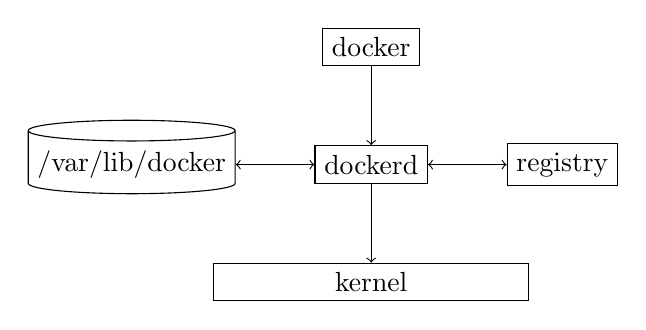
\begin{tikzpicture}
        \node[draw] (dockerd) {dockerd};
        \node[draw,above=of dockerd] (docker) {docker};
        \draw[->] (docker.south) -- (dockerd.north);

        \node[draw,right=of dockerd] (registry) {registry};
        \draw[<->] (dockerd.east) -- (registry.west);

        \node[cylinder,draw,
              shape border rotate=90,
              aspect=0.1,
              left=of dockerd] (lib_docker) {/var/lib/docker};
        \draw[<->] (dockerd.west) -- (lib_docker.east);

        \node[draw,below=of dockerd,minimum width=4cm] (kernel) {kernel};
        \draw[->] (dockerd.south) -- (kernel.north);
    \end{tikzpicture}
    \end{center}
\end{frame}


\begin{frame}[fragile]
    \frametitle{First containers}
    \begin{minted}{console}
# docker run ubuntu touch toto
# docker run ubuntu ls toto
ls: cannot access 'toto': No such file or directory
    \end{minted}
    \vfill
    hu ?
    \vfill
\end{frame}


\begin{frame}[fragile]
    \frametitle{First Image}
    \begin{minted}{console}
# cat Dockerfile
FROM ubuntu
RUN touch toto
# docker build . -t myimage
[...]
# docker run myimage ls toto
toto
    \end{minted}
\end{frame}

\begin{frame}[fragile]
    \frametitle{Container or image ?}
    \begin{columns}
    \begin{column}{0.45\textwidth}
	\begin{minted}[fontsize=\footnotesize]{console}
# docker run --name mycontainer \
    ubuntu touch toto
# docker commit mycontainer \
    --tag myimage
	\end{minted}
    \end{column}
    \begin{column}{0.45\textwidth}
	\begin{minted}[fontsize=\footnotesize]{console}
# cat Dockerfile
FROM ubuntu
RUN touch toto
# docker build . --tag myimage
        \end{minted}
    \end{column}
    \end{columns}
    \vfill
    {\it Containers} and {\it image} are the two sides of the same coin !
    \vfill
\end{frame}

\begin{frame}[fragile]
    \frametitle{Layers}
    \begin{center}
    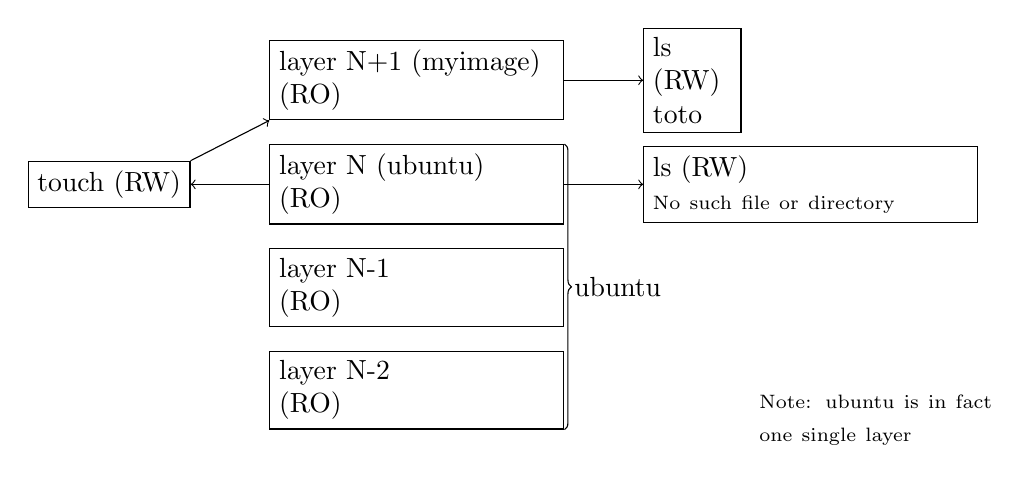
\begin{tikzpicture}
        \node[draw,text width=3.5cm]                        (myimage) {layer N+1 (myimage) \\(RO)};
        \node[draw,below=0.3cm of myimage,text width=3.5cm] (ubuntu3) {layer N (ubuntu) \\ (RO)};
        \node[draw,below=0.3cm of ubuntu3,text width=3.5cm] (ubuntu2) {layer N-1 \\ (RO)};
        \node[draw,below=0.3cm of ubuntu2,text width=3.5cm] (ubuntu1) {layer N-2 \\ (RO)};
        \node[draw,left=of ubuntu3]                       (touch)   {touch (RW)};
        \node[draw,right=of ubuntu3,text width=4cm]       (lsempty) {ls (RW) \\ {\scriptsize No such file or directory}};
        \node[draw,right=of myimage,text width=1cm]       (lstoto)  {ls (RW) \\ toto};
        \draw[->] (ubuntu3.west)     -- (touch.east);
        \draw[->] (touch.north east) -- (myimage.south west);
        \draw[->] (myimage.east)     -- (lstoto.west);
        \draw[->] (ubuntu3.east)     -- (lsempty.west);
        \draw[decorate,decoration=brace] (ubuntu3.north east) -- node[anchor=west](ubuntu){ubuntu} (ubuntu1.south east);
        \node[below right=of ubuntu, text width=3cm] {\scriptsize Note: ubuntu is in fact one single layer};
    \end{tikzpicture}

    \begin{itemize}
        \item Image = read-only
        \item Container = Image with an execution layer with possible read-write capabilities
    \end{itemize}
    \end{center}
\end{frame}

\begin{frame}[fragile]
    \frametitle{Commands on images}
    \begin{center}
    {\scriptsize
        \begin{table}
	    \begin{tabular}{|l|l|} \hline \rowcolor{lightgray}
Command                           & Action                                        \\ \hline
pull                              & Fetch image from registries                   \\ \hline
push                              & Push image to registries                      \\ \hline
tag                               & Add new tags to an image                      \\ \hline
rmi                               & Remove image from local storage               \\ \hline
images                            & List images                                   \\ \hline
history                           & Show layers info of an image                  \\ \hline
inspect                           & Display internal property of an image         \\ \hline
{\it build (take image tag as -t)} & Build image from Docker file (+ other image) \\ \hline
        \end{tabular}
        \end{table}
    }
    \vfill
    \begin{minted}{console}
[[docker.io[:443]/]library/]ubuntu[:latest]
    \end{minted}

    \begin{alertblock}{Tag}
    We often call $tag$ the last part (here: $latest$) but in docker command that's the whole name.
    \end{alertblock}
\end{center}

\end{frame}


\begin{frame}[fragile]
    \frametitle{Commands on containers}
    {\scriptsize
        \begin{table}
        \begin{tabular}{|l|p{5cm}|l|} \hline \rowcolor{lightgray}
Command       & Action                                        & Also do                   \\ \hline
run           & Run container from image                      & pull,create,start,attach  \\ \hline
ps            & List all container                            & -                         \\ \hline
logs          & Display stdout, stderr of container           & -                         \\ \hline
inspect       & Display internal status about container       & -                         \\ \hline
stop          & Stop a started container                      & -                         \\ \hline
kill          & Send signal to started container              & -                         \\ \hline
rm            & Remove a stopped container from disk          & -                         \\ \hline
create        & Create a stopped container from image         & pull                      \\ \hline
start         & Start a stopped container                     & -                         \\ \hline
diff          & Display change between container and it's image  & -                      \\ \hline
attach        & Display stdout, stderr \newline
                (+ pipe stdin and signal !) \newline
                of started container                          & -                         \\ \hline
commiy        & Freeze a container into an image              & -                         \\ \hline
        \end{tabular}
        \end{table}
    }
    \begin{center}
    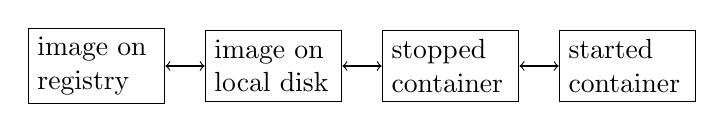
\begin{tikzpicture}
        \node[draw, text width=1.5cm] (registry) {image on registry};
        \node[draw, text width=1.5cm, right=0.5cm of registry] (localimage) {image on local disk};
        \draw[<->] (registry.east) -- (localimage.west);
        \node[draw, text width=1.5cm, right=0.5cm of localimage] (stoppedcontainer) {stopped container};
        \draw[<->] (localimage.east) -- (stoppedcontainer.west);
        \node[draw, text width=1.5cm, right=0.5cm of stoppedcontainer] (startedcontainer) {started container};
        \draw[<->] (stoppedcontainer.east) -- (startedcontainer.west);
    \end{tikzpicture}
    \end{center}
\end{frame}


\begin{frame}[fragile]
    \frametitle{Volumes}
    \begin{block}{Upgrade problem}
    I run a mysql 5.5 container with data in the container.

    But running a mysql 5.6 will create a fresh new container with no data
    \end{block}
    \begin{minted}[fontsize=\footnotesize]{console}
docker run --volume mysqldata:/var/lib/mysql --name mysql5.5 mysql:5.5
docker stop mysql5.5
docker run --volume mysqldata:/var/lib/mysql --name mysql5.6 mysql:5.6
    \end{minted}

    {\scriptsize
    \begin{table}
    \begin{tabular}{|l|p{5cm}|} \hline \rowcolor{lightgray}
Volume name                          & Volume location              \\ \hline
\mintinline{console}{mysqldata}      & somewhere in /var/lib/docker \\ \hline
\mintinline{console}{/var/lib/mysql} & /var/lib/mysql               \\ \hline
\mintinline{console}{./data}         & Does not work with docker ! \newline
                                       but works with docker-compose \\ \hline
    \end{tabular}
    \end{table}
    }
Except with path volume on Windows and Mac OS, there is huge performance gain using volume
\end{frame}

\begin{frame}[fragile]
    \frametitle{ENTRYPOINT \& CMD}

    \begin{columns}
    \begin{column}{0.48\textwidth}
        \begin{exampleblock}{Do}
        \begin{minted}{console}
ENTRYPOINT ['/bin/sh', '-c']
CMD ['./runserver.sh']
        \end{minted}
        \end{exampleblock}
    \end{column}
    \begin{column}{0.48\textwidth}
        \begin{alertblock}{Don't do}
        \begin{minted}{console}
RUN ['./runserver.sh']
        \end{minted}
        \end{alertblock}
    \end{column}
    \end{columns}

    \begin{table}
    \begin{tabular}{|l|l|p{4.5cm}|} \hline \rowcolor{lightgray}
ENTRYPOINT                          & Command (CMD)      & where                          \\ \hline
/docker.entrypoint.sh               & mysqld             & server process                 \\ \hline
['helm']                            & [--help]           & dedicated image for cli tools \newline
                                                           or programming language        \\ \hline
""                                  & bash               & OS image (ubuntu, centos)      \\ \hline
    \end{tabular}
    \end{table}

    \begin{block}{Forcing a shell to enter a server process container}
        \begin{minted}{console}
docker run -ti --entrypoint /bin/sh mysql
        \end{minted}
    \end{block}

\end{frame}

\begin{frame}[fragile]
    \frametitle{docker-compose}

    docker = imperative commands

    docker-compose = declarative file

    \vfill
    \begin{minted}{console}
# cat docker-compose.yaml
version: '3.4'

services:
  mycontainer:
    build: .
    volumes:
      - .:/workdir
    command: ["make", "-C", "slides"]
# docker-compose up
    \end{minted}
\end{frame}

\begin{frame}[fragile]
    \frametitle{Addendum: build cache}

    \begin{columns}
    \begin{column}{0.48\textwidth}
        \begin{alertblock}{Not optimize}
        \begin{minted}[fontsize=\footnotesize]{console}
FROM python
COPY . .
RUN pip install -r requirements.txt
        \end{minted}
        \end{alertblock}
    \end{column}
    \begin{column}{0.48\textwidth}
        \begin{exampleblock}{Optimized}
        \begin{minted}[fontsize=\footnotesize]{console}
FROM python
COPY requirements.txt .
RUN pip install -r requirements.txt
COPY . .
        \end{minted}
        \end{exampleblock}
    \end{column}
    \end{columns}

\end{frame}

\begin{frame}[fragile]
    \frametitle{Addendum: size of images}

    \begin{columns}
    \begin{column}{0.48\textwidth}
        \begin{alertblock}{Not optimized}
        \begin{minted}[fontsize=\footnotesize]{console}
FROM ubuntu
RUN apt-get install -y npm python
COPY package.json .
RUN npm build

RUN pip install -r requirements.txt
        \end{minted}
        \end{alertblock}
    \end{column}
    \begin{column}{0.49\textwidth}
        \begin{exampleblock}{Optimized}
        \begin{minted}[fontsize=\footnotesize]{console}
FROM node
COPY package.json .
RUN npm build
RUN pip install -r requirements.txt

FROM ubuntu # Second FROM !
RUN apt-get install -y \
    --no-install-recommends python \
 && rm -rf /var/lib/apt/lists/*
COPY requirements.txt .
RUN pip install --no-cache-dir -r requirements.txt
COPY . .
        \end{minted}
        \end{exampleblock}
    \end{column}
    \end{columns}
\end{frame}

\begin{frame}[fragile]
    \frametitle{\textcolor{red}{$X$ Appendix: anti-pattern 1/2 $X$}}

    \begin{minted}{console}
$ cat docker.entrypoint.sh
virtualenv venv                            <= Nope,
./venv/bin/pip install -r requirements.txt <= to move
webpack build                              <= at build time
chown www-data:www-data /var/lib/www
./env/bin/python ./manage.py runserver
    \end{minted}

\end{frame}

\begin{frame}[fragile]
    \frametitle{\textcolor{red}{$X$ Appendix: anti-pattern 2/2 $X$}}

    \begin{minted}{console}
CMD ['supervisord'] # run django, redis and mysql
    \end{minted}

    \vfill

    \textcolor{red}{Avoid running a process manager inside a container:}
    \begin{itemize}
        \item \textcolor{red}{logs of process manager are not really useful}
        \item \textcolor{red}{if pipe to stdout, unrelated logs are mixed together}
        \item \textcolor{red}{one composant die, are we notified ?}
    \end{itemize}
\end{frame}

\end{document}
